\section{Results: stage A}
\label{sec:results}

The numbers in this section are the stage A block of the pooled report.
Until that block is complete, each estimate is marked pending and no confirmatory sentence is promoted into the abstract.
Per-cell rows are in Appendix~\ref{app:cells}.

\subsection{Same rate, different fates}
\label{sec:h1}

H1 tests superiority of 0.05 for the shared-rule contrasts in E1: the two kit contrasts in every domain, plus the tolerance contrast in chain sum and in math, twelve contrasts in all.
The number that reject after Holm correction, among those with every completed seed positive, is $\HOneRejected{}$ of $\HOneFamily{}$.
H1-pooled is the equal-weight mean of each kit contrast across conclusive E1 cells.
The false-positive phrase contrast, resampled noise minus \texttt{fp\_trigger}, is $\HOnePooledTrigger{}$ (one-sided $p = \HOnePooledTriggerP{}$).
The false-negative phrase contrast, resampled noise minus \texttt{fn\_behavior}, is $\HOnePooledFn{}$ (one-sided $p = \HOnePooledFnP{}$).
H2 is the equivalence family on the ten prompt-specific contrasts, at the same margin of 0.05.
Its decision is confirmatory and is stated in the abstract only if the family passes.
The chain-sum decoy is reported beside H1 and is outside the family.
% AFTER-RESULTS: (H1 holds) At least one shared rule separates from rate-matched noise by more than the margin.
% AFTER-RESULTS: (H1 does not hold) No shared-rule contrast clears the margin on the preregistered test.
% AFTER-RESULTS: (H1-pooled holds) The kit effect is not a single domain.
% AFTER-RESULTS: (H1-pooled does not hold) The equal-weight kit contrasts do not clear zero.
% AFTER-RESULTS: (H2 holds) Prompt-specific errors are equivalent to resampled noise at the margin.
% AFTER-RESULTS: (H2 does not hold) At least one prompt-specific contrast is outside the equivalence margin.

\subsection{The screen orders fates}
\label{sec:h3}

H3 is the Spearman correlation, over stage A's non-withdrawn matched pairs, between the locked gap in transfer precision and the gap in endpoint accuracy.
The rate is equal inside each pair by construction, so step-0 $J$ cannot produce the correlation, and the null permutes gaps within cells, so differences in overall accuracy between cells cannot produce it either.
The pooled within-pair correlation is $\HThreeRho{}$ (permutation $p = \HThreeP{}$, 5th percentile $\HThreeQFive{}$, $n = \HThreeN{}$).
Figure~\ref{fig:h3} is that scatter, with natural pairs marked.
% AFTER-RESULTS: (H3 holds) The locked screen orders endpoint accuracy on the stage A pairs.
% AFTER-RESULTS: (H3 does not hold) The locked screen does not order endpoint accuracy on the preregistered test.

\begin{figure}[t]
\centering
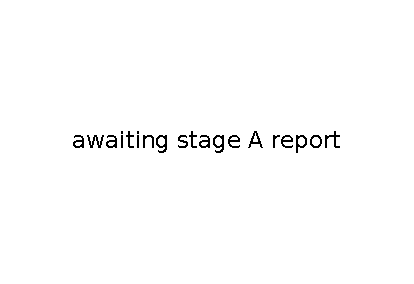
\includegraphics[width=\columnwidth]{figures/fig_h3.pdf}
\caption{Stage A matched pairs. The horizontal axis is the locked gap in transfer precision and the vertical axis is the gap in endpoint held-out oracle accuracy. Natural pairs are diamonds. Each pair shares one step-0 rate, so $J$ is constant within a pair.}
\label{fig:h3}
\end{figure}

The same pairs are scored by baselines that do not use the screen, and by the structure label that the theory assigns without a statistic: $-1$ for a shared-behaviour rule and $0$ otherwise.
Table~\ref{tab:baselines} reports each baseline's correlation with the accuracy gap and the gap $\rho(\tau) - \rho(b)$.
The class baseline correlates at $\HThreeClassRho{}$, and $\rho(\tau) - \rho(\mathrm{class})$ is $\HThreeClassGap{}$.
Inside the stratum of shared and natural pairs, where the structure label assigns no direction, the correlation is $\HThreeSharedRho{}$ (permutation $p = \HThreeSharedP{}$, 5th percentile $\HThreeSharedQFive{}$, $n = \HThreeSharedN{}$).
The audit that produces $J$, the precisions, the cosine, the probe, the Egashira product, and the screen is shared by every arm in the cell.
The step-25 baseline is one short training run per arm.
% AFTER-RESULTS: (class gap is positive and H3 holds) The screen orders pairs that a shared-versus-other label does not separate.
% AFTER-RESULTS: (class gap is not positive) The structure label accounts for as much of the ranking as the screen on this sample.
% AFTER-RESULTS: (shared stratum holds) The ordering remains inside the shared and natural pairs.
% AFTER-RESULTS: (shared stratum does not hold) The ordering does not remain once the sample is restricted to shared and natural pairs.

\begin{table*}[t]
\caption{Baselines for the stage A accuracy gaps. $\rho$ is the baseline's Spearman correlation. The last column is where the number comes from. The note under the table is the break-even count of verifiers.}
\label{tab:baselines}
\centering
\small
\setlength{\tabcolsep}{4pt}
\begin{tabular}{lrrp{0.28\textwidth}}
\toprule
Baseline & $\rho$ & $\rho(\tau)-\rho(b)$ & Cost \\
\midrule
step-0 Youden J & \pending & \pending & shared audit \\
mean precision & \pending & \pending & shared audit \\
modal precision & \pending & \pending & shared audit \\
$\cos(g_V, g_O)$ & \pending & \pending & shared audit \\
held-out probe AUC & \pending & \pending & shared audit \\
step-25 accuracy & \pending & \pending & one 25-step run per verifier \\
Egashira et al.\ $f \times C$ & \pending & \pending & shared audit \\
shared-behaviour label & \pending & \pending & rule label, no training \\
\bottomrule
\end{tabular}

The audit, with its features, is paid once per cell and serves every verifier; a step-25 run is one short training job per verifier. From recorded wall time, one audit costs as much as \BreakEvenMeasured{} step-25 runs. No projected ratio is quoted: the plan does not price the audit's gradient pass.

\end{table*}

\subsection{Same class, opposite direction}
\label{sec:h10}

H10 holds the structure class fixed.
For each pair $(a, b)$ the estimate is the equal-weight mean over conclusive E1 cells of $\mathrm{sign}(\Delta\tau)\,(\mathrm{acc}_a - \mathrm{acc}_b)$, with the locked $\Delta\tau = \tau_{\mathrm{pool}}(a) - \tau_{\mathrm{pool}}(b)$.
The pairs are $(\texttt{fp\_trigger\_enriched}, \texttt{fp\_trigger})$ and $(\texttt{fn\_behavior\_depleted}, \texttt{fn\_behavior})$.
The aligned gaps are $\HTenTrigger{}$ (one-sided $p = \HTenTriggerP{}$) and $\HTenFn{}$ (one-sided $p = \HTenFnP{}$), with Holm correction across the two pairs and a minimum of three cells.
A negative $\Delta\tau$ flips the accuracy gap before the average, so a rule that merely says shared errors are bad cannot pass.
Only the direction the screen reads can.
% AFTER-RESULTS: (H10 holds) The screen separates two shared phrase rules that have the same rate and the same class.
% AFTER-RESULTS: (H10 does not hold) The screen does not separate the same-class phrase pairs on the preregistered test.

\subsection{Natural verifiers and patching}
\label{sec:h7}

H7 tests whether a natural verifier differs from resampled noise at its own rate.
The family has five pairs: two in math, and one each in code, instruction following, and judged question answering.
The number of those pairs whose interval excludes zero is $\HSevenNDiff{}$.
For every pair that differs, the sign of the contrast is compared with the sign of the locked transfer-precision gap.
Figure~\ref{fig:natural} plots each natural verifier's step-0 error rate, $\mathrm{FPR} + \mathrm{FNR} = 1 - J$, against that locked gap and against the endpoint accuracy gap.
H8 is the patch comparison on the domains where the two selections differ.
The equal-weight mean of screen patch minus error-count patch is $\HEightPoint{}$ (one-sided $p = \HEightP{}$, $n = \HEightN{}$ domains).
% AFTER-RESULTS: (H7 holds) At least one natural verifier separates from rate-matched noise.
% AFTER-RESULTS: (H7 does not hold) The natural verifiers do not separate from rate-matched noise on the preregistered test.
% AFTER-RESULTS: (H8 holds) Choosing the two categories by the screen beats choosing them by the error count.
% AFTER-RESULTS: (H8 does not hold) The screen's patch does not beat the error-count patch.

\begin{figure*}[t]
\centering

\includegraphics[width=\textwidth,height=1.55in,keepaspectratio]{figures/fig_natural.pdf}
\caption{Natural verifiers in stage A. Each point is one natural verifier. The horizontal axis is its step-0 error rate, $\mathrm{FPR} + \mathrm{FNR} = 1 - J$. The vertical axes are the locked transfer-precision gap and the endpoint accuracy gap, both as natural minus its resampled control. If rate decided fate, every point would sit at zero on both vertical axes.}
\label{fig:natural}
\end{figure*}

\subsection{How many oracle labels}
\label{sec:h9}

H9 recomputes the stage A correlation from the stored draws of $\tau_{\mathrm{pool}}$ at 32, 64, 128, and 192 labels.
Draws are not imputed.
The median correlations are $\HNineMedThirtyTwo{}$, $\HNineMedSixtyFour{}$, $\HNineMedOneTwoEight{}$, and $\HNineMedOneNineTwo{}$.
The 5th percentiles are $\HNineQThirtyTwo{}$, $\HNineQSixtyFour{}$, $\HNineQOneTwoEight{}$, and $\HNineQOneNineTwo{}$.
The fractions of draws with positive correlation are $\HNinePosThirtyTwo{}$, $\HNinePosSixtyFour{}$, $\HNinePosOneTwoEight{}$, and $\HNinePosOneNineTwo{}$.
Figure~\ref{fig:h9} plots the medians.
H9 is secondary.
% AFTER-RESULTS: (the median rises toward 192) Extra labels past the smallest budget move the screen.
% AFTER-RESULTS: (the median is flat) The smaller budgets already match the 192-label screen on this sample.

\begin{figure}[t]
\centering
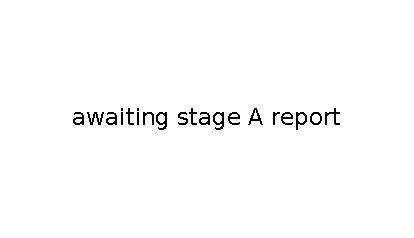
\includegraphics[width=\columnwidth,height=1.55in,keepaspectratio]{figures/fig_h9.pdf}
\caption{Oracle-label budget for the stage A screen. The curve is the median correlation of the stored $\tau_{\mathrm{pool}}$ draws with the endpoint accuracy gap, at each number of oracle labels.}
\label{fig:h9}
\end{figure}
